% Chapter 4 is usually termed 'Concept', 'Design' or 'Model'. Here you describe your approach, give a
% high-level description to the architectural structure and to the single components that your solution
% consists of. Use structured images and UML diagrams for explanation. This chapter will have a volume
% of 20-30 percent of your thesis.
%
% This chapter introduces the architectural design of Component X. The component consists of
% subcomponent A, B and C.
%
% In the end of this chapter you should write a specification for your solution, including
% interfaces, protocols and parameters.

\chapter{Concept\label{cha:concept}}

This section will explain in more detail the concepts of each individual component and how they will
play together. They individually contribute to the overall goal of implementing a development and
test automation platform to build HbbTV applications. The DevTools Backend service will be the base
component and will help us to achieve the first part of building a state of the art web-authoring
experience. It enables new possibilities for developers to inspect an HbbTV app and understand and debug
JavaScript problems within the code. It helps to instrument the application and also to run automated
WebDriver tests with the Appium HbbTV Driver. This component acts as translator between the WebDriver
protocol and the Remote Debugging Protocol. To do that on a bigger scale we need the Raspberry Pi to
deploy that driver to any TV without any manual steps. To manage all these driver we then use a
Selenium Grid and with a proper CI/CD server we can leverage that setup to test and release our HbbTV
apps faster and with more confidence.

\section{Components\label{sec:components}}

\subsection{DevTools Backend\label{sec:devtoolsbackend}}

The DevTools Backend is the main component of the overall design. It has to do most of the work
and is the only component that directly interacts with the targeted environment: the HbbTV
application. Debugging an HbbTV application these days is almost impossible. Even though some TV
manufactures provide some interfaces and APIs to connect to the TV they are barely documented and
almost different for each TV model. To provide a tool that covers all TVs of all manufactures, it
requires a different approach than hooking into a native interface. Until all manufactures recognize
the demand for developers to get a better development support this won't change. We already had a
similar situation a couple of years ago when the smart phone market started to explode and a lot of
people started writing mobile or hybrid apps for Android and iOS. At that time both vendors had
almost no support for any debugging tools that would help developers to inspect the page. A tool
called \textit{Weinre}\footnote{WEb INspector REmote - \url{http://people.apache.org/~pmuellr/weinre/docs/latest/Home.html}}
was developed and found a lot of popularity within the developer community. It enabled to debug
arbitrary web pages remotely for the first time, especially on a mobile device such as a phone. It
used a unique approach that allowed to do that for all mobile environments (Android, iOS and Hybrid
web applications run by PhoneGap/Cordova). After vendors started to support remote debugging natively
due to the success of this project it became obsolete and the inventor stopped maintaining it.

This project is the role model for the DevTools Backend component. Similar how it allows to remote
debug applications for smartphones, the DevTools Backend will allow it for HbbTV based apps on Smart
TVs. The idea is simple. A script that gets executed within a targeted environment connects to a
server to exchange information and commands as utility for a 3rd party authoring tool. The concept works
independant from the environment and device. As long as the target supports basic web technology
like HTML and JavaScript it will run everywhere. So this component can not only be used to debug HbbTV
apps on Smart TVs but also to inspect any other IoT device like a fridge or a coffee machine as long
as their interfaces are based on web technologies\footnote{Infact the screen in the Tesla Model S
is build on top of a proparitary web browser and therefor all Tesla apps are build with web
technology. Theoretically the DevTools Backend can be used to debug these apps with modern web
authoring tools already today.} \footnote{An example application can be found here: \url{http://dash.time4tesla.com/}}.

The component itself consists of two subcomponents. Similar to \textit{Weinre} it has a frontend
part that takes care on instrumenting the target environment and a backend part which is a server
that initializes and manages the data traffic between target environment and authoring tool. Both
subcomponents have logic to handle methods or trigger events according to the Remote Debugging
Protocol. As stated in section \ref{sec:remotedebuggingprotocol} the Remote Debugging Protocol is
supported by all WebKit browser and has first class support for one of the most used web authoring
tools these days: the Chrome DevTools. In addition to that it is actively maintained by a dedicated
team at Google and is well documented\footnote{\url{https://chromedevtools.github.io/devtools-protocol/}}.
In order to provide as much integration without any additional effort it only makes sense to rely on
a well maintained protocol like this.

When it comes to debugging an HbbTV application there will be always three parties involved. The
instrumentation logic, the backend and the authoring tool. The instrumentation logic is what actually
interacts with the target environment. It executes commands that it receives from the backend and
returns desired information. Since the instrumentation script is not much more than any other script
on the page it can't support all methods that are defined within the Remote Debugging Protocol.
However the JavaScript API is pretty comprehensive and covers the essential requirements of that
protocol like returning and modifying the state of certain properties like e.g. DOM nodes. Many things can
be emulated which is sufficient for this use case. It is important to ensure that the instrumentation
script doesn't affect in any way other scripts or the web application in general from behaving
differently. It has to keep its environment as pristine as possible. As a debugging tool it should
help developers to find bugs and not create them. Once an instrumentation script was injected
into the environment it has to register itself to the backend. Script and backend establish their
connection via WebSockets. Since events and methods will be exchanged randomly from both sides
it is important to have a full duplex connection type so both ends can communicate with each other
in an asynchronous fashion. To identify the target, the instrumentation script has to identify
itself with an unique id that can be either the host of the HbbTV app or a random chosen string. The
backend will register the page based on that id and some other metadata and will manage any
connections to it so that arbitrary clients can connect to the page with the backend as proxy. Due
to some house keeping work the backend will never directly connect a client to the instrumented
page. In fact it will manage the communication with two different WebSocket channels. Not all method
requests from clients are directed to the page itself. For example all methods of the Remote Debugging
Protocol that relate to network events or page lifecycles are handled by the backend. Figure
\ref{fig:command_handling} shows the activity between all parties in more detail.

\begin{figure}[htb]
  \centering
  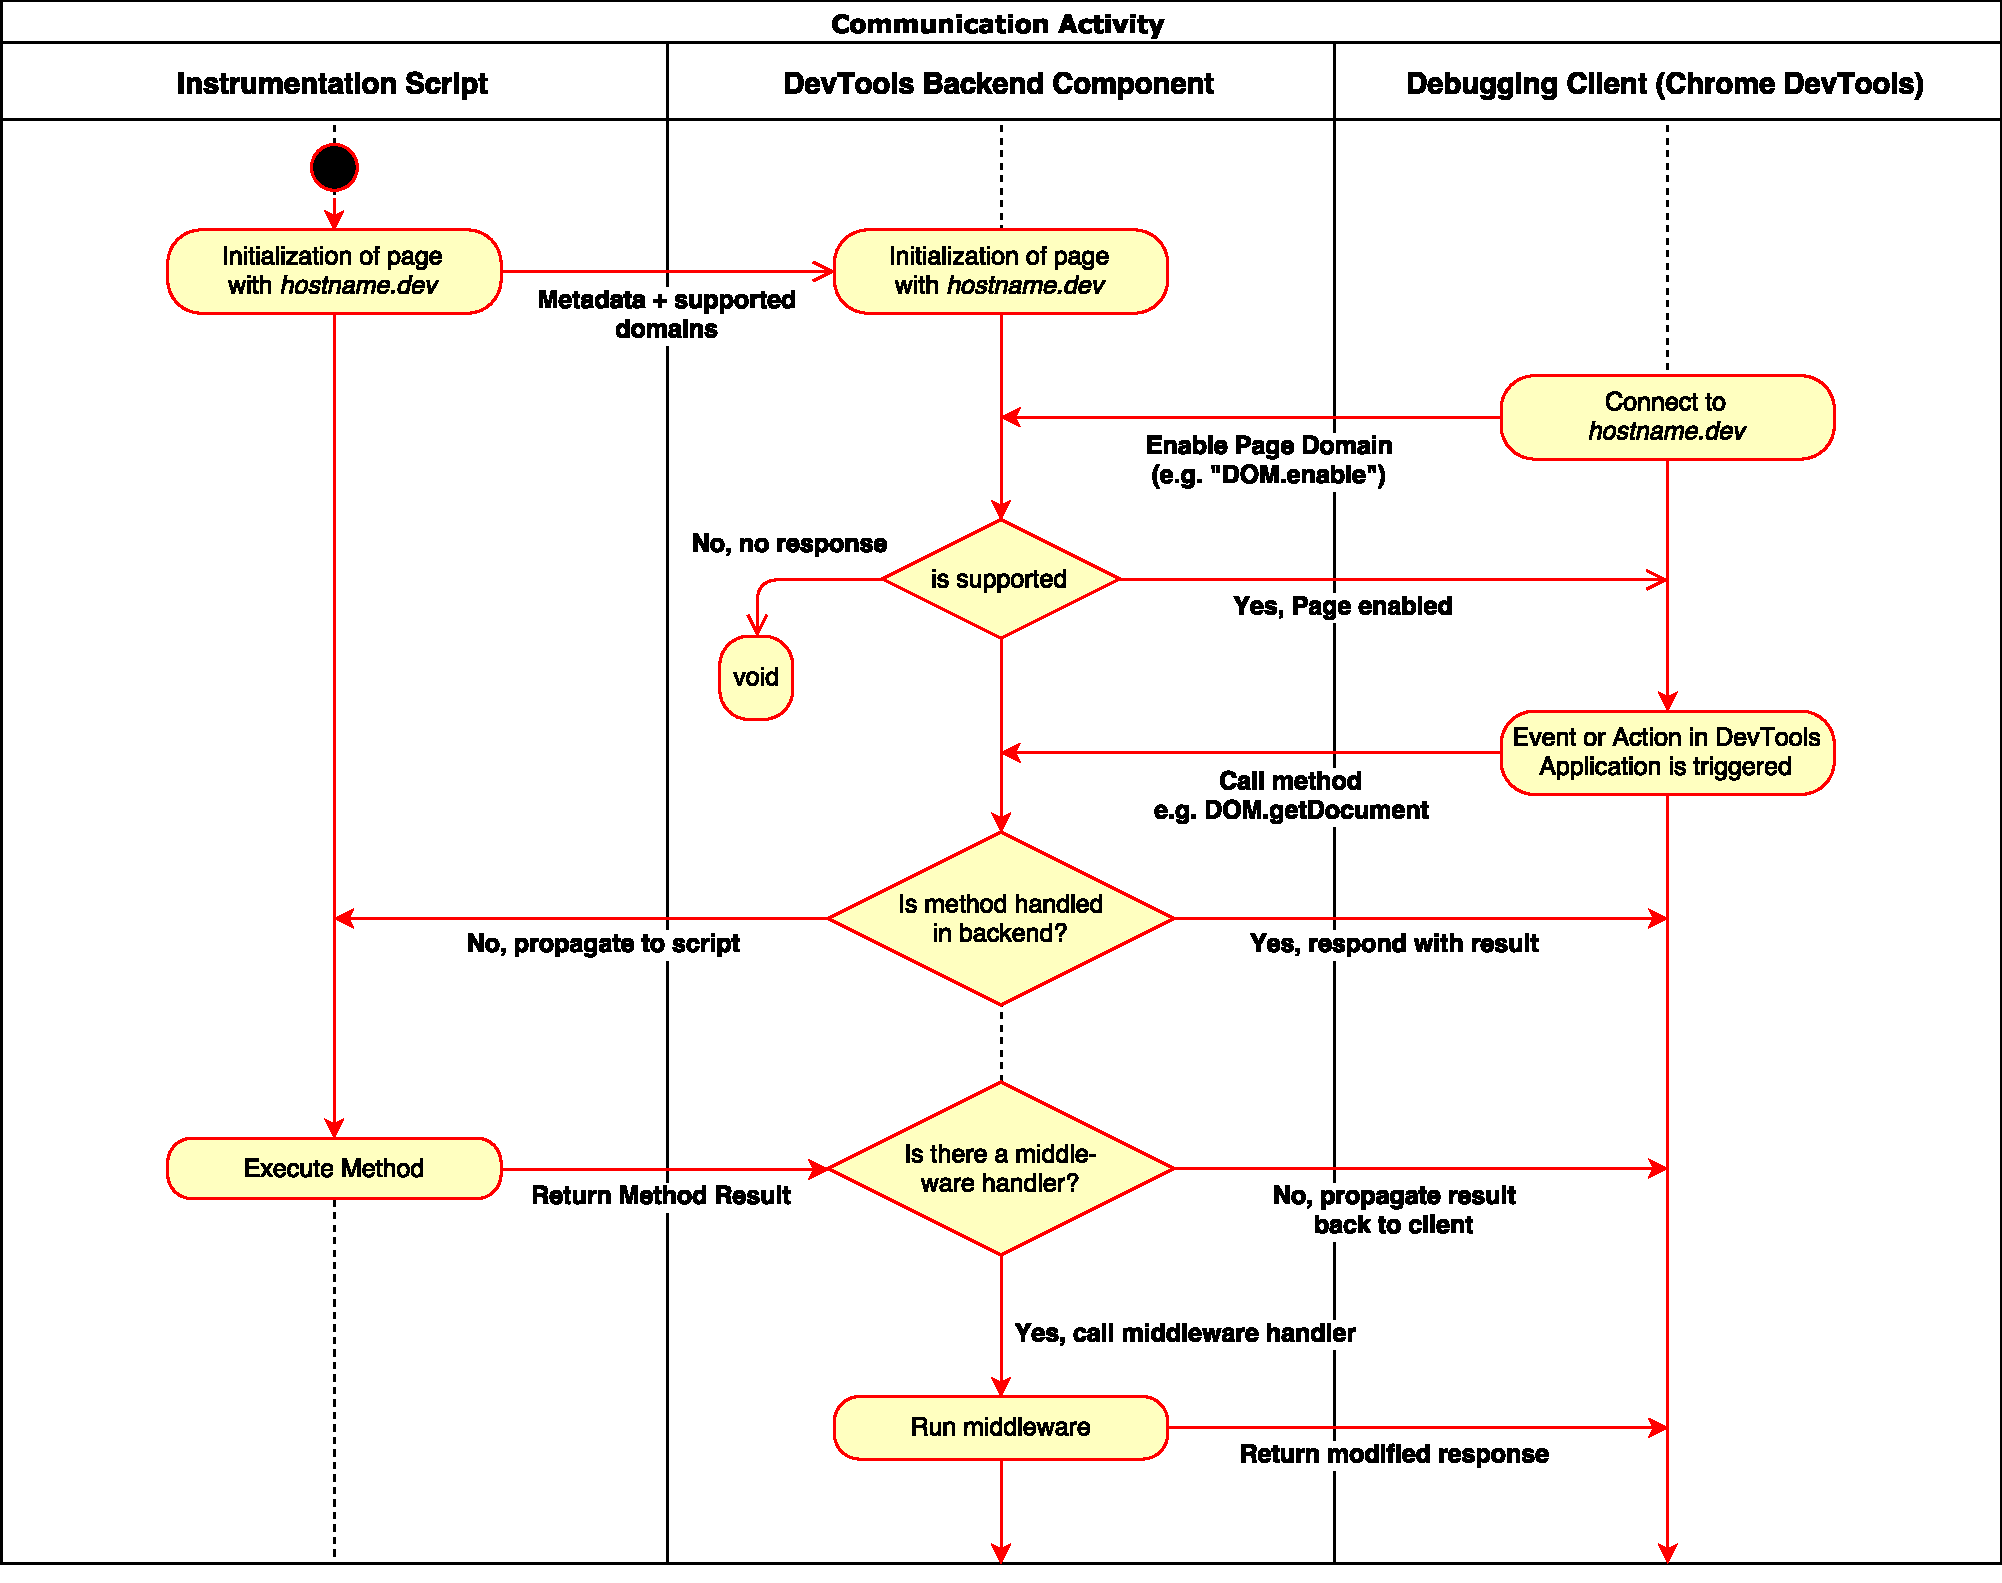
\includegraphics[width=15cm]{command_handling.pdf}\\
  \caption{Communication Activity between Instrumentation Script, Backend and Debugging Client}\label{fig:command_handling}
\end{figure}

In scenarios where a full page load happened the instrumentation script looses the connection with
the backend. It manages to reconnect to the target, given that the page unique id is still the same,
and makes sure it propagates the right lifecycle events to the connected clients. They won't recognise
any connection abruption and instead properly handle the page load on their side. In some cases the
response of the instrumentation script needs to be enhanced with data from the backend. This happens
when network data is involved which is only stored on the backend side. A middleware handles this
situation by enhancing the result object before returning it back to the client.

There are two ways to inject the instrumentation script into the target environment. It can be either
placed manually into the page by referencing the script via script tag or the DevTools Backend can be
used as a proxy. In this case it captures all http packages on a certain port (usually port 80) and
injects the script inline into the page automatically. The proxy registers the page to the backend
based on the data it gets from the request. This has the advantage that the application doesn't have
to get modified to instrument it. However running the target device (e.g. the Smart TV) through a
proxy is not always possible. Therefor the component provides a launcher script that can connect to
the backend to register the page before the instrumentiation script gets initiated.

Once this happened and a remote debugging client connects to the backend they both exchange JSON
payload over the socket channels. The client usually listens to certain domain events (depending
of the use case) and fires methods with an id, a method name containing the domain and the request
(e.g. \textit{CSS.getMatchedStylesForNode}) as well as some parameters that get propagated to the
method (e.g. a node id). Each domain has to get enabled by the debugging client so that the
communication can be reduced to the minimum. If the client would enable all domains it would
overflow the socket channels. This keeps the data amount manageable. The backend only propagates
messages to the instrumentation script if the containing method was enabled by the client
beforehand. Even though all methods and events of the protocol are documented in a comprehensive
way\footnote{see \url{https://chromedevtools.github.io/devtools-protocol/}} the order of events
and methods that have to get triggered on both sides is unknown. The only way to find out when
certain events has to get thrown is by debugging the debugging tool. Since the Chrome DevTools
is just a normal web-application it is possible to debug it using the Chrome DevTools itself.
Within the \textit{Timeline} tab it is possible to inspect the WebSocket connection to the browser
in real time. This allows to reverse engineer the protocol and emulate a similar behavior like in
the browser.

\subsection{Appium HbbTV Driver\label{sec:appiumhbbtvdriver}}

Based on the DevTools Backend component the Appium HbbTV Driver is now able to run its automated
tests without having to take care about how to automate WebDriver commands on the TV. Since the
DevTools Backend is applicable to all HbbTV supported devices the driver can therefor be utilised
on arbitrary TVs or SetUp boxes supporting that format. It uses the already existing framework
utilities provided by Appium to support all common functionalities that an automation driver
requires. Appium already provides a variety of drivers that are mainly focused on mobile automation.
However its vision is to create more drivers that support new devices and platforms. HbbTV is the
perfect fit for that. With Appiums Basedriver module\footnote{\url{https://github.com/appium/appium-base-driver}}
it provides not only a template to build the driver but also comes with all required features to
run it on bigger scale e.g. within a Selenium Grid out of the box. An overview about all involved
components is shown in figure \ref{fig:hbbtv-driver-components}.

\vspace{1cm}
\begin{figure}[htb]
  \centering
  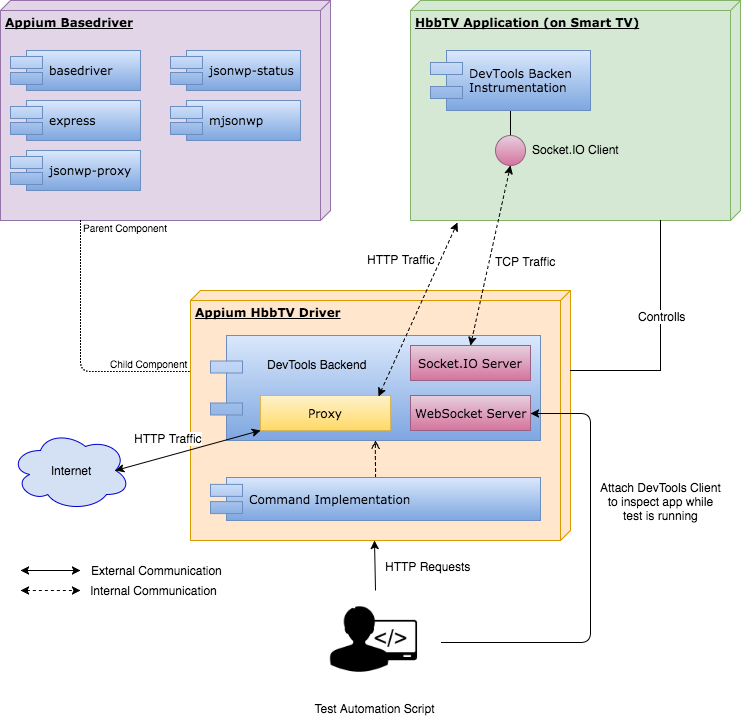
\includegraphics[width=15cm]{hbbtv-driver-components.png}\\
  \caption{Appium HbbTV Driver components}\label{fig:hbbtv-driver-components}
\end{figure}
\vspace{0.5cm}

Thanks to Appiums Basedriver a lot of important functionality can be inherited. It builds the
foundation of the actual driver. It takes care of session management and capability definition/validation
(\textit{''basedriver''}), provides predefined WebDriver routings (\textit{''mjsonwp''}) which are
served by a preconfigured HTTP server component (\textit{''express''}). With that it manages incomming
HTTP requests and handles their responses by applying the correct response codes (\textit{''jsonwp-status''}).
That also allows additional features like proxying these requests (\textit{''jsonwp-proxy''}).
Since it is using the Appium framework on one side and the DevTools Backend on the other the only
task of this driver is to translate the WebDriver commands into the Remote Debugging Protocol.
WebDriver commands are send as normal HTTP requests. The driver acts as a restful HTTP server
and can receive these request. Depending on the endpoint it triggers a different action on the
target device. Every automated test starts by initating a WebDriver session. Figure 4.2 demonstrates
this process in detail.

\vspace{1cm}
\begin{figure}[htb]
  \centering
  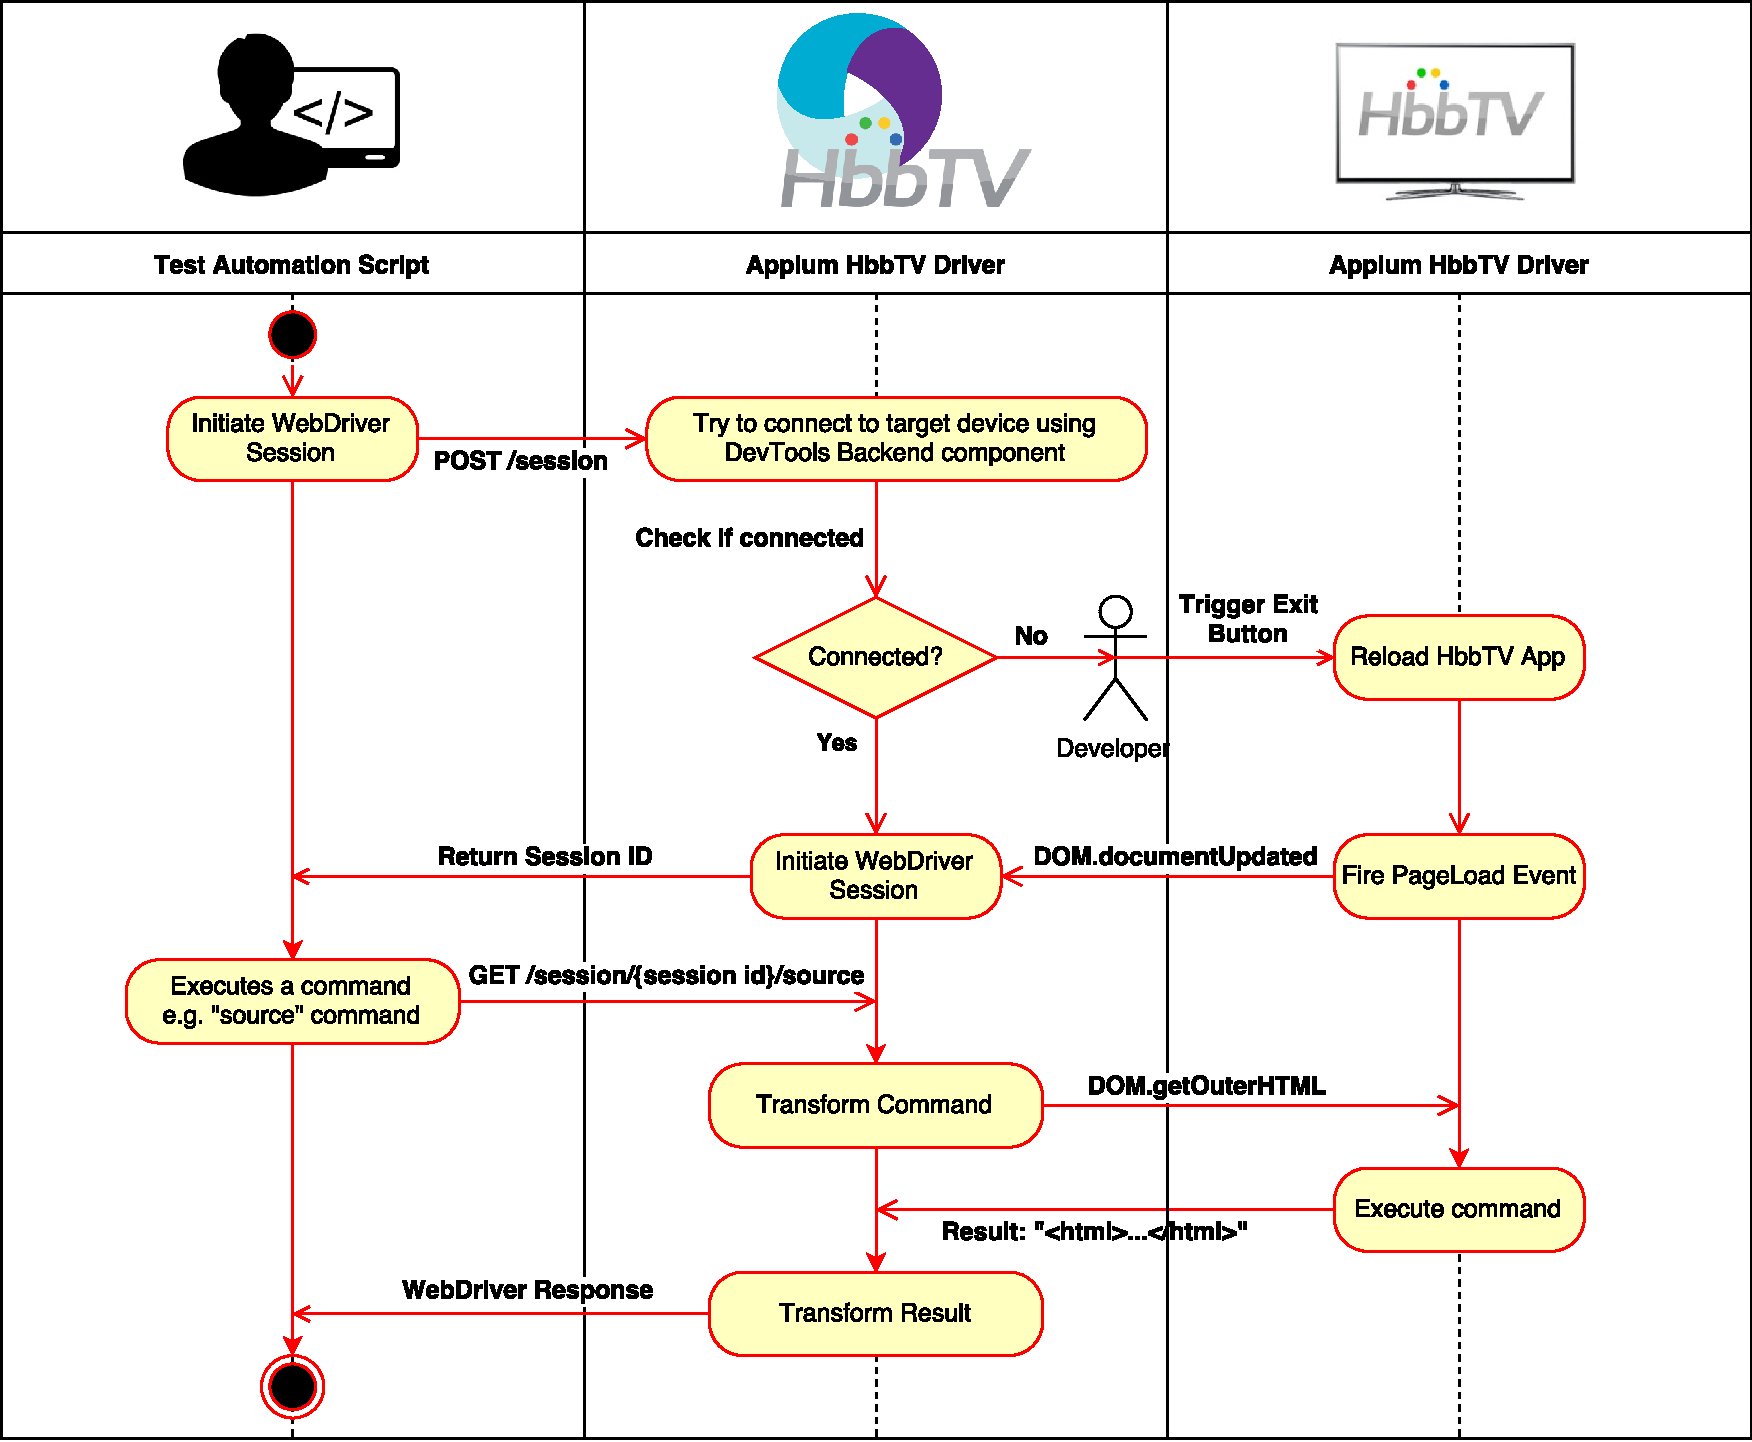
\includegraphics[width=15cm]{appium-driver-diagram.pdf}\\
  \caption{Creating A WebDriver Session}\label{fig:appium-driver-diagram}
\end{figure}
\vspace{0.5cm}

A session can only be successful initiated if the DevTools backend component is able to successfully
connect to the target device. In case the TV is turned off or never got instrumented by the DevTools
Backend it requires one manual step to finish the initiation process. By pressing the Exit button
on the remote the HbbTV app gets reloaded and the DevTools Backend can inject the script if used as
a proxy. If the instrumentation script is injected manually the test script can connect to it by
providing the page ID within its capabilities. Once a connection to the target device was established
the initial session request can be resolved. The response includes a session ID next to other
information of the assigned device. The session ID is important as it is part of almost all WebDriver
endpoints to identify the user and execute all commands on the right device.

Depending on the test framework of the developer the session ID gets automatically stored within the
test context. The developer can now run any WebDriver commands. After the driver has received a new
command it transforms it into a Chrome DevTools Protocol method and forwards it to the DevTools
Backend component. Since the Dev- Tools Backend is using an asynchronous socket connection the driver
has to wait until either the result of the method was returned or a certain event was triggered in
order to resolve the WebDriver HTTP request. Certain commands can trigger a page load in the target
environment that will break the connection between the DevTools Backend component and the instrumentation
script. In these cases the driver has to wait until a reconnection happened in order to resolve the
request, otherwise the test script would not be able to send the next command. If the connection can't
be re-establised a timeout will be hit and causes to return with an error.

\subsection{Raspberry Pi\label{sec:pi}}

To ensure that such connection lost never happens a man in the middle component between network and
Smart TV can be used. A peripheral like a Raspberry Pi\footnote{https://www.raspberrypi.org/} is
an ideal utility to manage a TVs network traffic and instrument any HbbTV app on the fly. A
Raspberry Pi is a \textit{''fully customizable and programmable small computer board''}\cite{raspberrypi}
with a size of a credit card. It has a 1.2GHz 64-bit quad-core ARMv8 processor with 1 GB RAM,
4 USB and 1 Ethernet port. It is known as the mainstay in the world of makers and electronics but
also as an educational device that brings people the joy of electronics and computer programming.
With 38\euro{} it is super cheap and yet powerful. People who are familar with Linux have no problems
to start building tools and applications with it. With a prebuild Raspbian operating system the
provisioning of a TV to test HbbTV apps can be reduced to a simple plug\&play step.

The idea is that all network traffic of the Smart TV runs through the Raspberry Pi. Running
the DevTools Backend component it acts as a Proxy between TV and network. This has the advantage
that every HbbTV app will be instrumented on the fly. There is no need to manually inject an
instrumentation script. The DevTools Backend proxy modifies every HTTP packages that has an HbbTV
mime type before it sends it back to the TV. In addition to that it tracks all application assets
so that the developer can inspect all files that have been downloaded by the HbbTV app including
information like request and response headers. This setup allows to not only do that with own
applications but also with any HbbTV app of any broadcaster that can be received by the Smart TV.
Having said that it allows to monitor all communications between HbbTV app and server and helps
to understand how certain application track your behavior while using the app.

In order to put this together, it requires an additional ethernet cable as well as an USB to Ethernet
adapter. The Raspberry Pi has to maintain two network interfaces. One is for the data transfer between
TV and Pi and the other for the one between Pi and network. Therefor you could theoretically also use
the Wifi module to connect to your network instead of using the USB adapter. With the correct network
setup it should connect automatically. Once it is connected to the power supply the operating system
boots up and starts the Appium HbbTV Driver. To identify the Raspberry Pi we change the hostname
settings to be the model name of the TV it is connected to. After the Pi has established a connection
between TV and our network we can immediately address this host as our automation server and run tests
on it.

\vspace{1cm}
\begin{figure}[htb]
  \centering
  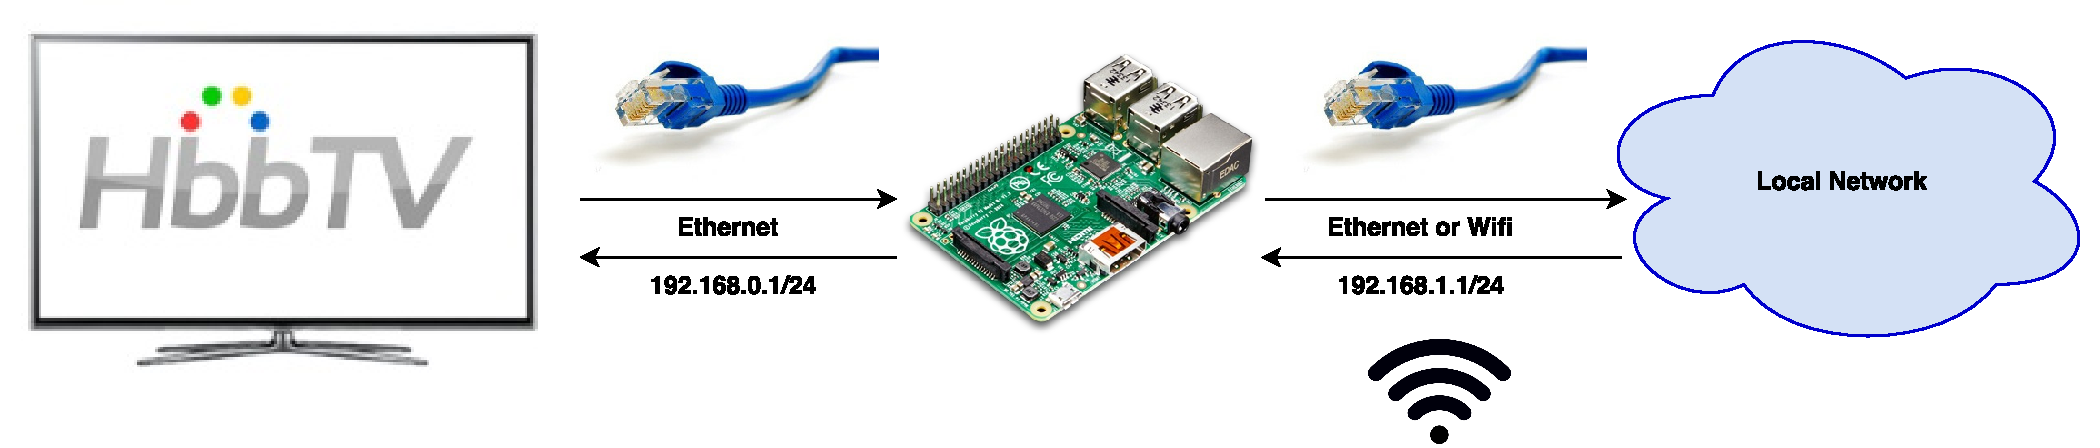
\includegraphics[width=15cm]{pisetup.pdf}\\
  \caption{Setup of SmartTV with Raspberry Pi}\label{fig:pisetup}
\end{figure}
\vspace{0.5cm}

To seperate the network traffic we have to run both interfaces on different subnets. This can be
customised depending on the given network. Most local networks will have an IP range of
\textit{192.168.1.1/24} which is why this setup would make the most sense as default. However
once a proper network is found it is possible to copy the images to other Raspberry Pis. This will
allow us to provision an already existing TV lab in a simple way and deploy our components to run
automated WebDriver tests using the Appium HbbTV Driver and DevTools Backend.

\section{Selenium Grid\label{sec:grid}}

To run our automated tests on multiple TVs with different HbbTV support at the same time we need
a Selenium Grid to orchastrate the WebDriver requests. The Appium HbbTV Driver component allows us
to register to such a grid using an internal settings page that the user can open in the browser.
The only information that is required is the IP address of the Selenium Grid server. That server
has to be accessible in the network where the TV and the Raspberry Pi are located in. The driver
will send a request to the Selenium Grid server containing the capabilities of the TV. It is
important that the DevTools Backend is able to connect at least once with an HbbTV app to identify
the TV. It could also just use the provided API of the TV. However this is different depending on
the manufacture and the TV model. To cover this within this thesis would be out of scope but an
interesting feature for the future. If the registration to the grid server was successful it will
automatically ping the Raspberry Pi every once in a while to check its connectivity.

\vspace{1cm}
\begin{figure}[htb]
  \centering
  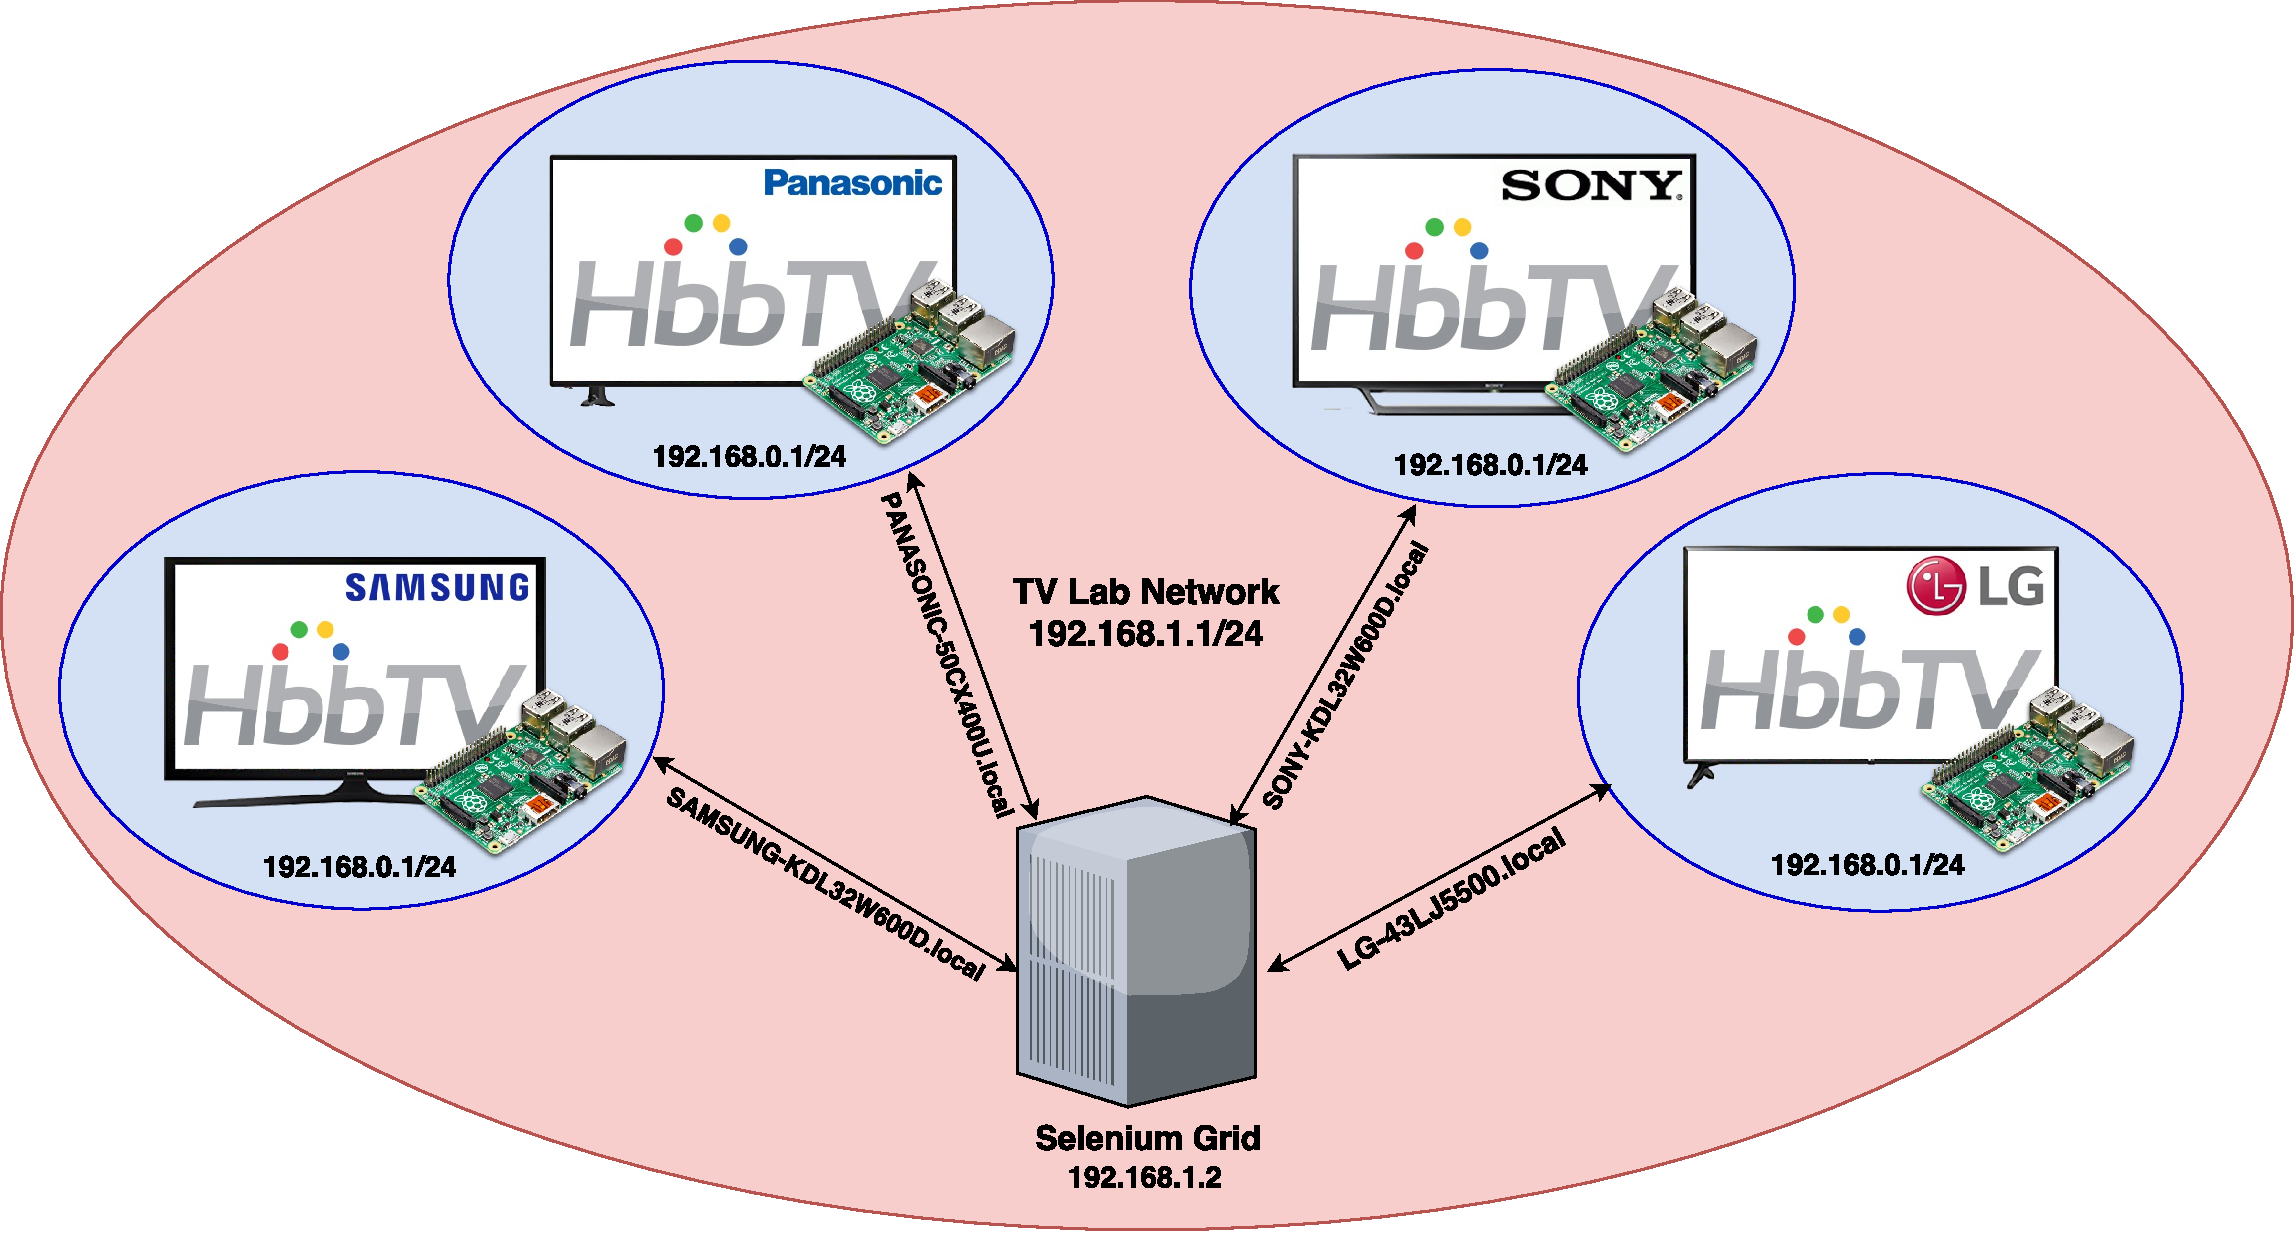
\includegraphics[width=15cm]{network.pdf}\\
  \caption{Network Setup of TV Lab with Raspberry Pi}\label{fig:network}
\end{figure}
\vspace{0.5cm}

The Selenium Grid will be the access point for all developers to run their automated tests on. It
manages its capabilities and only creates a session if the desired device is available and not used
by someone else. If a device is blocked due to another test it will queue up the request and waits
until it becomes available again. Each Smart TV is registered with the supported HbbTV version, the
name of the manufacture and its model name. Each test can therefor specify on what kind of device
it should be running. The Selenium Grid tries to find the best suiteable device if available. If for
example the developer wants to run a test on a Smart TV with supported HbbTV 1.5 the grid server
randomly selects a Smart TV that runs that HbbTV version. The same goes for other capabilities. All
data about registered Smart TVs and their availability can also be consumed as JSON blob using
the Rest API of the grid server. This allows to create custom dashboards that are more aligned to
the TV theme. Instead of just model names it could display the TV model as image with the manufacture
logo.

\section{Continuos Integration and Delivery\label{sec:cicd}}

The last step to have a fully automated continuous integration and delivery pipeline is to setup
an automation server that runs our tests as soon as any code changes were introduced to the project.
There are mutliple ways to setup such pipeline. CI/CD became a major part in the software delivery
process over the last years so that many tools have been developed since then. One of the most
popular open source solutions is Jenkins\footnote{\url{https://jenkins.io/}}. It is \textit{''deployed
at large scale in many organizations''}\cite{jenkins} and \textit{''has no licensing costs''}\cite{jenkins}.
In combination with a source control tool like Git\footnote{\url{https://git-scm.com/}} we can
trigger our automated tests regularly so that defects are detected at early stage before it is
deployed to production. Depending on the project and its requirements you can deploy different
strategies on how code gets tested and pushed to a production environment. This can be fully automated
so that no human interaction is necessary anymore.

% ToDo: explain CI/CD process of HbbTV app
